%   Filename    : chapter_2.tex 

\chapter{Review of Related Literature}
\label{sec:relatedlit}


\section{Automatic Speech Recognition}
\label{sec:ASR}

Automatic Speech Recognition (ASR) is a technology that processes human speech into readable text by the use of machine learning or artificial intelligence (AI). The ASR system has grown popular over the past decade as it quickly approaches human accuracy levels, there is a great demand for applications taking advantage of ASR technology in their products to make audio and video data more accessible \shortcite{Foster:2023}.

Automatic Speech Recognition independently decodes and transcribes spoken language using a machine-base process. An ASR system takes in acoustic signals from a speaker via a microphone, analyzes these signals using various patterns, models, or algorithms, and generates an output, most commonly in text form \shortcite{Levis:2012}. The importance of differentiating speech recognition from speech understanding (speech identification) is that, speech understanding focuses on interpreting the meaning of an utterance rather than merely transcribing it. Furthermore, speech recognition is distinct from voice recognition: speech recognition pertains to a machine's capability to identify the words spoken, while voice recognition relates to a machine's ability to discern the manner of speaking \shortcite{Levis:2012}.

\section{Lexicon Model}
\label{sec:LexiconModel}

The lexicon model is essential in automatic speech recognition, serving as the bridge between the acoustic representation and the sequence of words produced by the speech recognizer. The lexicon's function can be viewed in two aspects: it first identifies the words or lexical items recognized by the system, and second, it offers the framework to develop acoustic models for each entry \shortcite{Adda-Decker:2000}. Consequently, lexical design consists of two primary components: determining and selecting the vocabulary items and representing each pronunciation entry using the fundamental acoustic units of the recognizer. In large vocabulary speech recognition, the vocabulary is typically chosen to optimize lexical coverage within a specified size of the lexicon, and the basic units selected are generally phonemes or phone-like units (\shortcite{Adda-Decker:2000}.

\section{Acoustic Model}
\label{sec:AcousticModel}
Acoustic modeling is a fundamental and preliminary step in the process of speech recognition. The acoustic model defines the relationship between acoustic data and linguistic elements. Most calculations in acoustic modeling are attributed to feature extraction and statistical representation, making it a crucial factor in the recognition process. Statistical representations are derived from the features that have been extracted \shortcite{Bhatt:2020}. In the acoustic model, the distribution of these extracted features corresponding to specific sounds is modeled to create a connection between the features and the structures of the linguistic units. 

According to \shortciteA{Bhatt:2020}, several techniques for feature extraction, including those based on human perception and the mechanics of voice production, have been documented. Features were derived for acoustic modeling in a speaker-independent recognition context since such systems pose challenges in speech recognition.

\section{Language Model}
\label{sec:LanguageModel}
Language models are crucial for various daily applications, including correcting grammatical errors, recognizing speech, and summarizing text. Due to the recent advancements in deep learning techniques, conventional n-gram and word embedding language models are being substituted with neural network-based models \shortcite{Mago:2020}.

Large Language Models (LLMs) have recently shown remarkable abilities, encompassing tasks like natural language processing (NLP), language translation, text generation, and answering questions. In addition, LLMs play a vital role in computerized language processing, capable of grasping intricate verbal patterns and producing relevant and coherent responses in various contexts. However, the significant advancements in LLMs have led to a surge in research contributions, making it challenging to fully comprehend the overall impact of these developments \shortcite{Fahad:2024}.

\section{Local Dialects and Low-Resource Languages On Automatic Speech Recognition}
\label{sec:LocalDialects}
Deep learning technologies have evolved from rudimentary systems to advanced models that can fluently comprehend natural language, making remarkable progress in their integration into Automatic Speech Recognition (ASR). Neural networks have become crucial in ASR for capturing temporal dynamics and phonetic differences, enabling wider use in virtual assistants, educational applications, and customer support \shortcite{Alharbi:2021}. Noisy environments where background sounds significantly impair the accuracy and dependability of speech recognition. The considerable challenge for languages with limited resources is the size of the vocabulary. This influences the performance of the model in which larger vocabularies enhance adaptability but demand more data and computational power. ASR systems struggle with dialectal variation, which can impede model accuracy due to differences in pronunciation, a concern for languages such as Akeanon, known for its various dialects \shortcite{Alharbi:2021}. 

Initial attempts to make Philippine speech corpora were restricted by their size, scope, and lack of multilingual data. The creation of speech technology for low-resource Philippine languages was hindered by these limitations. The DOST-funded ISIP project developed the Philippine Languages Database (PLD) was developed by \shortcite{Cajote:2023} to solve this. This includes more than 453 hours of reading and casual conversations in 10 different languages, such as Filipino, Cebuano, Hiligaynon, and others. The PLD enables the development of ASR, TTS, phoneme transcription, and voice conversion systems. PDL is a useful tool to enhance language technology and educational resources in the Philippines due to its parallel and multilingual design.

\section{The Kaldi ASR Toolkit}
\label{sec: KALDI}
The structure of Kaldi, an open-source toolkit available for speech recognition research, is examined. Kaldi offers a speech recognition framework built on finite-state transducers, utilizing the freely accessible OpenFst, along with comprehensive documentation and scripts for constructing entire recognition systems.
\shortciteA{Povey:2011} characterized Kaldi as a contemporary toolkit for speech recognition. It is built to be flexible and features one of the more permissive licenses, which enhances its accessibility. Numerous research works have utilized Kaldi in their applications.

\section{The Basic Language Resource Kit}
\label{sec: BLARK}
The Basic Language Resource Kit (BLARK) is a framework designed to give and provide a minimal set of resource language that is required in conducting pre competitive research and education in language and speech technology \shortcite{Krauwer:2003}. This concept is important in languages that are underrepresented, this helps researchers and developers address the gaps in linguistic resource availability and advances in technology. The framework ensures that underrepresented languages that often lack commercial interest are not forgotten in the global information society. 
The target audience for BLARK are researchers, both in academia and in industry, and educators. The framework is used as a material to train students for research of pilot experiment and applications. It is important to have tools for production and annotation of a new corpus and source format for all modules and resources available when using BLARK, to make industrial developers freely adapt and use the framework to the specific requirements of their application.

\section{The Akeanon Language}
\label{sec:AkeanonLanguage}
\subsection{History and its Speakers}
\shortciteA{Zorc:1995} stated that Akeanon serves as the main language in the northwestern area of Panay Island in the central Philippines, boasting over 350,000 speakers. Both the language and its speakers derive their name from the Akean River, which runs through the heart of the province by the same name. The people, culture, and items linked to this river and region are referred to as Aklanon, while the language is known as Inakeanon, incorporating the -in- infix and an accent alteration, or more generally Bisaya, as Aklanons identify themselves as part of the Visayan cultural and linguistic family. Many Aklanons, particularly those in professional fields, have relocated to various major cities in the Philippines, such as Manila, Iloilo, and South Cotabato \cite{AkeanonMap}, in pursuit of job opportunities, with sizable communities also found in San Francisco and New York. Figure~\ref{fig:akeanonmap} shows a heatmap of Akeanon-speaking households all over the Philippines. The dialect discussed here is that of Kalibo, Aklan, the provincial capital and its main commercial hub. Other dialects are linked to the towns of Altavas, Batan, Balete, Banga, Madalag, New Washington, Numancia, Malinao, Lezo, Makato, Tangalan, Nabas, Ibajay, and Libacao—though the latter two show significant divergence, they remain mutually understandable with the others. Two towns exist within Aklan province that feature different dialects—with Buruanga associated with Kinaray-a, and Malay linked to various dialects of Tablas, Romblon. The closest languages to Akeanon are Kinaray-a and Kuyonon, both of which belong to the West Bisayan subgroup of Central Philippine languages.

\begin{figure}[h!]
	\centering
	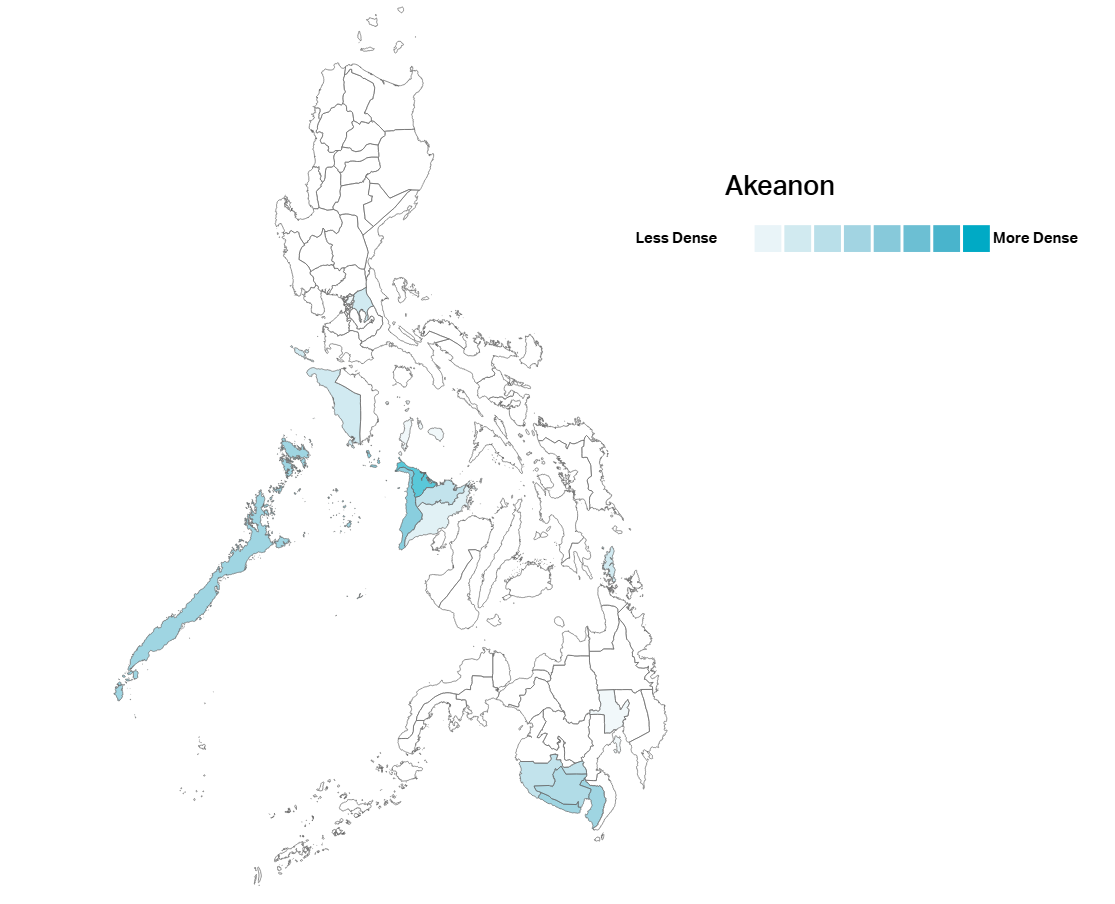
\includegraphics[width=\textwidth]{./figures/akeanon-map.png}
	\caption{Geographic distribution of Akeanon-speaking households in the Philippines.}
	\label{fig:akeanonmap}
\end{figure}

\subsection{Phonology}
\textbf{Akeanon Phonology: Historical and Synchronic Perspectives}
  
The Akeanon language, native to the Aklan province in the Philippines, possesses a distinctive phoneme that sets it apart from other Philippine-type languages. Initially recognized as a voiced velar fricative and subsequently categorized as a velar approximant, this phoneme differentiates Akeanon from its linguistic siblings within the Bisayan group, such as Hiligaynon, Cebuano, and Kinaray-a. Subsequent research by \shortciteA{deLaCruz:1968} characterized it as a voiced velar fricative, functioning both as a consonant and a semivowel. More recent studies have reiterated its classification as a velar approximant, emphasizing its absence of articulatory turbulence \shortcite{Zorc:1995, Rentillo:2022}. Table~\ref{tab:vowel_inventory} shows the Akeanon vowel inventory defined by \shortciteA{Zorc:1995} while Table~\ref{tab:consonant_inventory} shows the updated consonant inventory for the Akeanon language argued by \shortciteA{Rentillo:2022}. It is worth noting that consonantal sounds enclosed in parentheses indicate that these sounds are not fully integrated in the Akeanon phonetic system but they appear in limited context such as names and argot.

\begin{table}[H]
   \centering
   \caption{Vowel Inventory for Akeanon}
   \label{tab:vowel_inventory}
   \renewcommand{\arraystretch}{1.5} % AdjuSst row height
   \begin{tabular}{|l|c|c|c|}
       \hline
        & \textbf{Front} & \textbf{Central} & \textbf{Back} \\ 
       \hline
       \textbf{Close} & \textipa{i \textasciitilde I} &  & \textipa{u \textasciitilde o} \\ 
       \hline
       \textbf{Open-Mid} & (\textepsilon) &  & (\textopeno) \\ 
       \hline
       \textbf{Open} & \multicolumn{2}{c|}{\textipa{a \textasciitilde \textturna}} & \\ 
       \hline
   \end{tabular}
\end{table}


\begin{table}[H]
   \centering
   \caption{Updated Consonant Inventory for Akeanon} \vspace{0.25em}
   \label{tab:consonant_inventory}
   \renewcommand{\arraystretch}{1.2} % Adjust row height for better spacing
   \setlength{\tabcolsep}{5pt} % Reduce horizontal padding

   \resizebox{\textwidth}{!}{ % Resize to fit within text width
   \begin{tabular}{|l|c|c|c|c|c|c|c|}
      \hline
      & \textbf{Bilabial} & \textbf{Alveolar} & \textbf{Post-Alveolar} & \textbf{Palatal} & \textbf{Velar} & \textbf{Labiovelar} & \textbf{Glottal} \\ 
      \hline
      \textbf{Stop} & p, b & t, d &  &  & k, g &  & \textipa{P} \\ 
      \hline
      \textbf{Nasal} & m & n &  &  & \textipa{N} &  &  \\ 
      \hline
      \textbf{Affricate} &  & (\textipa{ts}), (\textipa{dz}) & (\textipa{tS}), (\textipa{dZ}) &  &  &  &  \\ 
      \hline
      \textbf{Fricative} & (\textipa{f}), (\textipa{v}) & \textipa{s}, (\textipa{z}) & (\textipa{S}) &  &  &  & \textipa{h} \\ 
      \hline
      \textbf{Approximant} &  &  &  & \textipa{j} &  & \textturnmrleg & \textipa{w} \\ 
      \hline
      \textbf{Tap} &  &  \textfishhookr &  &  &  &  &  \\ 
      \hline
      \textbf{Lateral} &  & \textipa{l} &  &  &  &  &  \\ 
      \hline
   \end{tabular}
   } % End resizebox

\end{table}


\textbf{Linguistic Status and Usage of Akeanon }
 
Akeanon is acknowledged as an institutional language according to the Expanded Graded Intergenerational Disruption Scale (EGIDS) and is included in the Mother Tongue-Based Multilingual Education (MTB-MLE) program in primary education. With approximately 500,000 speakers based on recent estimates, the language flourishes in both spoken and written forms, encompassing social media, radio programs, and public signages. Its phonological framework, which is defined by a three-vowel inventory and distinctive consonantal reflexes, has been influenced by historical changes and cross-linguistic interactions.

\textbf{Cross-linguistic Comparisons and Historical Accounts}
  
The evolution of the Akeanon phoneme is believed to reflect more extensive linguistic trends, such as velarization and palatalization, seen in various languages. \shortciteA{Rentillo:2022} contend that the development of the phoneme may have been shaped by regional linguistic changes or historical interactions with other Bisayan dialects. Moreover, historical accounts from figures such as \citeA{Aparicio:1841} and \citeA{Monteclaro:1929} indicate cultural and linguistic connections to Borneo, which influenced the distinct characteristics of Akeanon speech.

\textbf{Acoustic and Articulatory Characteristics}  

Recent acoustic studies conducted by \shortciteA{Rentillo:2022} offer empirical insights that differentiate the velar approximant from other phonemes. Their research demonstrates that the formant frequencies (F1 and F2) of this phoneme are lower than those of vowels, with variations that depend on adjacent phonological contexts. These findings emphasize the phoneme's unique articulatory properties, confirming its classification as an approximant rather than a fricative.

\textbf{Implications for Language Documentation}  

The distinctive attributes of Akeanon phonology reinforce the significance of documenting endangered and lesser-known languages. The Akeanon phoneme acts as a case study for exploring phonological diversity and innovation within Philippine languages. As noted by \shortciteA{Rentillo:2022}, further research could yield greater understanding of the historical and sociolinguistic elements that influence such unique linguistic features.

\subsection{Morphology}

\textbf{Morphology and its Role in Language}

Morphology, which examines word structures and their smallest meaningful units, is fundamental to comprehending the formation and development of languages. In various languages, including Akeanon, derivational morphology transforms syntactic roles or introduces novel meanings through methods like affixation, reduplication, subtraction, and internal modification of words. These methods not only redefine lexical meanings but also influence word categories like parts of speech \shortcite{Biray:2023}.

\textbf{Linguistic Diversity in the Philippines}

The Philippines is distinguished by its extensive linguistic variety, containing over 180 distinct languages, predominantly of Austronesian origin. Akeanon, which has approximately 460,000 speakers, belongs to the Malayo-Polynesian language family and functions as an official language in the province of Aklan. The language shares lexical similarities with Kinaray-a and Kuyunon, accompanied by notable dialectical variations throughout the area.

\textbf{Akeanon Dialectical Variations}

Akeanon dialects—including common Akeanon, Buruangganon, Nabasnon, and Bukidnon—display specific linguistic characteristics. These dialects are shaped by their geographical and cultural backgrounds, resulting in differences in structure, word order, and affixation. For example, reduplication serves as a prominent morphological feature that modifies meanings, whereas circumfixes are frequently utilized for the formation of new words. Dialect-specific phonemic variations, such as replacing "l" with "r" in certain instances, further highlight these distinctions.

\textbf{Social and Cultural Significance}

The Akeanon language mirrors the social traits of its speakers, showcasing values such as hospitality and respect. Expressions of endearment and polite language are prevalent in daily interactions, emphasizing the cultural identity of the community. Despite structural differences, the fundamental meanings of expressions remain uniform across dialects, illustrating the language’s strength and flexibility.

\textbf{Challenges and Preservation Efforts}

Like many other languages in the Philippines, Akeanon faces challenges stemming from modernization and the growing impact of technology. Initiatives to safeguard the language include its integration into the Mother Tongue-Based Multilingual Education (MTB-MLE) framework and the creation of orthographies that document its linguistic characteristics. Nonetheless, further support from both local and national organizations is crucial to maintain and promote the language in the face of the rising influence of global languages.

\subsection{The 300 Languages Project: A Worldwide Linguistic Initiative}
The 300 Languages Project, led by The Rosetta Project and The Long Now Foundation, stands as a groundbreaking effort aimed at creating a universal collection of human languages. This project seeks to gather and digitize parallel text and audio data from the 300 most frequently spoken languages around the globe. This extensive initiative addresses the significant shortage of resources for linguistic research, particularly for lesser-known languages, by utilizing volunteer-submitted public domain texts and recordings, all of which will be made available through The Internet Archive.

\textbf{Linguistic Variety and Digital Visibility}

Among the roughly 7,000 languages spoken worldwide, merely 20-30 languages possess a substantial digital footprint, including English, Spanish, and Mandarin. These languages, in conjunction with the next 270-280 most spoken languages, encompass over 90\% of the global populace. In contrast, the remaining 10\% communicate in one of the 6,700 minority languages, many of which are at risk of extinction due to inadequate digital and physical documentation. The 300 Languages Project highlights the importance of showcasing these minority languages by establishing a scalable "seed corpus" that begins small but is intended to expand sustainably.

\textbf{Contributions to Multilingual Research and Technological Advancements}

This initiative distinguishes itself by merging linguistic preservation with technological innovation. By assembling a large-scale public domain multilingual parallel corpus, the project enables progress in speech recognition, automated translation, and cross-linguistic studies. The absence of such resources has historically limited research and development to a small number of languages with existing corpus. The project’s focus on widely translated texts, such as the Swadesh List, the Universal Declaration of Human Rights, and chapters 1-3 of Genesis, ensures extensive applicability for linguistic research and tech applications.

\textbf{Volunteer-Driven, Scalable Approach}

The project's dependence on volunteer-contributed materials highlights its scalability and cost-efficiency. By establishing a comprehensive protocol for language documentation, this effort lays out a replicable model for documenting additional languages beyond the initial 300. The low-cost, community-focused method reflects earlier successful documentation endeavors like the ancient Rosetta Stone, which facilitated the understanding of Egyptian hieroglyphs through parallel texts.

\textbf{Significance for Language Conservation}

The 300 Languages Project plays a crucial role in preserving linguistic diversity by documenting and archiving minority languages that are on the brink of disappearing. By making multilingual resources publicly accessible, the initiative not only benefits researchers but also bolsters educational and cultural preservation efforts worldwide. Its alignment with the ALLOW initiative at the Language Technologies Institute further demonstrates a collaborative dedication to advancements in speech and language technologies.

\begin{comment}
\section{Chapter Summary}
Should include a table of related studies comparing them based on several criteria.

Highlight research gaps and the research problem.
\end{comment}


